\begin{itemize}
\item Syntetizace fotorealistických obrazů je oblastí PG, která dovoluje vykreslit jakoukoliv uměle vytvořenou scénu tak, jak by vypadala v reálném světě. 
\item Toho dosahuje díky implementaci optických zákonů, které lze běžně pozorovat.
\end{itemize}

\subsection{Sledování paprsku - ray tracing}
\begin{itemize}
 \item Metoda sleduje šíření paprsků ve scéně.
 \item Tyto paprsky začínají \textbf{ve světelném zdroji}, \textbf{odráží} se o tělesa v prostoru a některé z nich nakonec dopadnou do průmětny (obdobně jako světlo v reálném světě).
 \item Paprsky, které takto prochází scénu, lze znázornit jako strom.
 \item Tento přístup je však \textbf{neefektivní}, protože \textbf{velká část paprsků do průmětny nikdy nedopadne}, takže nemají přínos pro výsledný obraz a zbytečně zvyšují výpočetní čas.
\end{itemize}
\begin{figure}[H]
\centering
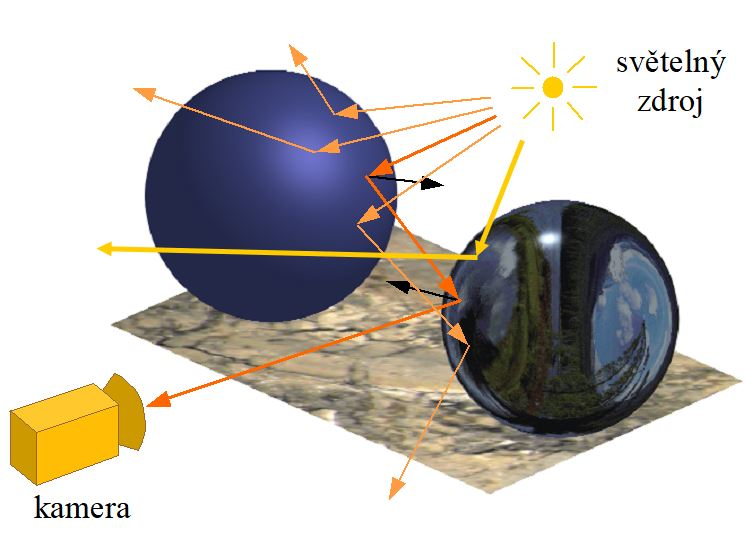
\includegraphics[width=0.6\textwidth]{assets/6_ray_trace_svetlo}
\end{figure}

\subsection{Zpětné sledování paprsku}
\begin{itemize}
 \item Funguje stejně jako běžné sledování paprsku, ovšem paprsky jsou \textbf{vysílány z kamery do scény}.
 \item Jakmile paprsky dosáhnou \textbf{ukončovacího kritéria} (jdou mimo scénu/maximální počet odrazů), sledujeme zpět jejich pohyb (navrácení z rekurze) a vypočítáváme osvětlení.
 \item Tím se eliminuje možnost, že by paprsek nepřinesl žádný přínos výslednému obrazu a značně se tak urychluje celý proces ray tracingu.
\end{itemize}
\begin{figure}[H]
\centering
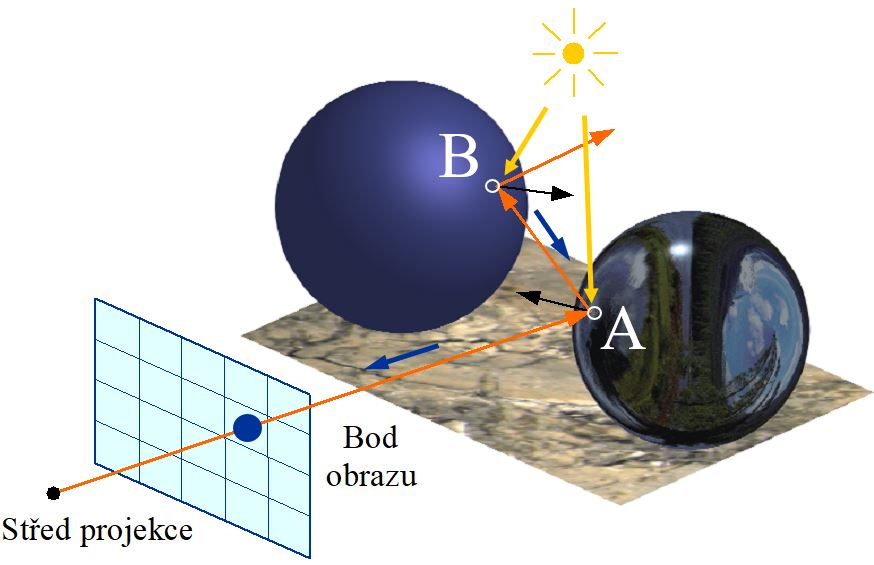
\includegraphics[width=0.6\textwidth]{assets/6_ray_trace_kamera}
\end{figure}

\subsection{Rekurzivní sledování paprsku}
\begin{itemize}
 \item Metoda vyšetřuje \uv{běh} světelných paprsků ve scéně.
 \item Světlo je reprezentováno \textbf{paprsky}, které jsou do scény vyzařovány světelnými zdroji a \textbf{putují prostorem} scény, některé dopadnou na povrchy těles, jiné odletí ze scény.
 \item Paprsek, který dopadne na povrch tělesa se může \textbf{odrazit} (zákon odrazu) nebo pokud je těleso průhledné, může se paprsek \textbf{zlomit} (zákon lomu) -- oba druhy paprsků mohou opět dopadnout na povrch těles, kde se celý proces znovu opakuje. %bitč
 \item Do scény se vyšle \textbf{velké množství paprsků}, ale podstatné jsou ty, které projdou objektivem myšlené kamery, pokud na průmětnu dopadne dostatečný počet paprsků, vykreslí se obrázek.
\item Metoda je sice jasná a fyzikálně podložená, ale nepoužívá se, protože se obtížně realizuje. (Je potřeba vyslat velké množství paprsků, ale k objektivu kamery by jich dorazilo jen malé množství a ostatní by se sledovaly zbytečně). 
\item Řešením je \textbf{otočit paprsky a vyslat je od kamery ke světelnému zdroji}. Principiálně to pak funguje stejně.
% \item Rekurzivní sledování paprsku funguje na tom principu, že jakmile primární paprsek (z kamery do průmětny) dopadne na nějaký objekt, dojde v tomto místě k jeho odrazu/lomu, ověří se, zda je bod dopadu osvětlen a vypočte lokální osvětlení (Phongův osvětlovací model).
% \item Na základně možného odrazu a lomu se do scény vysílají sekundární paprsky, které zapříčiní potřebnou rekurzi.
% \item Tato rekurze umožní trasovat např. průhlednost.
% \item Zároveň však prodlužuje výpočetní nároky.
% \item Hloubka rekurze se zpravidla nastavuje napevno.
 \begin{figure}[H]
		\centering
		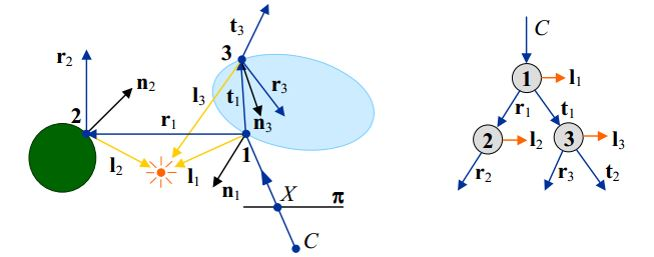
\includegraphics[width=0.6\textwidth]{assets/6_rekurzivni_sledovani_paprsku}
\end{figure}
 \item Rovnice výpočtu lokálního osvětlení: $I = I_l + k_rI_r + k_tI_t$ \\
  $I_l = I_aO_a + \sum\limits_{i} S_if_{att_i}I_i(O_d \cos{\varphi_i} + O_s \cos^n{\alpha_i} )$.
	Hodnota Si představuje viditelnost i-tého zdroje světla v daném bodě.
\end{itemize}
\subsection{Urychlování trasování}
Největším problémem je hledání průsečíků paprsků s objekty scény.
\begin{enumerate}
\item Nejjednodušším řešením je využít \textbf{ohraničujících ploch} (\uv{bounding boxů}). Ohraničující plocha se vytvoří kolem každého objektu ve scéně. Nejlépe když má plocha následující vlastnosti
\begin{itemize} 
	\item objekt leží \textbf{celý uvnitř} ohraničující plochy, ale plocha jej obepíná co \textbf{nejtěšněji},
	\item průsečíky paprsků s plochou musí jít spočítat, co nejjednodušším výpočtem,
	\item plochu musí být možné pro jednotlivé objekty dostatečně jednoduše nalézt.
\end{itemize}
Je možné použít \textbf{kulovou plochu} (ne moc vhodné, objekty můžou být protáhlé a tato plocha by je neobepínala dostatešně těšně). Další variantou plochy je \textbf{kvádr} (taky sice není moc vhodný, protože těleso může být našikmo a taky by jej neobepínal moc natěsno, nicméně nalezení ohraničující plochy je snadné -- minimální a maximální hodnoty obepínaného tělesa).
\begin{figure}[H]
\centering
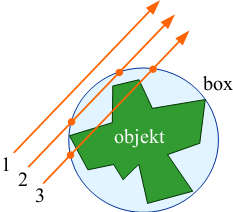
\includegraphics[width=0.2\textwidth]{assets/6_boudingbox}
\end{figure}
Princip ohranučujících ploch spočívá v tom, že pokud paprsek neprotne ohraničující plochu, pak neprotne ani těleso uvnitř (velmi časté). Odhalením této situace dojde ke značnému zrychlení. Pokud je to naopak, hledají se průsečíky s ohraničeným tělesem.
\item Rozšířením předchozího je \textbf{organizování ohraničujících ploch do hierarchických struktur}. Princip je stejný, pokud se neprotne rodičovská plocha, nehledají se dále ani průsečíky s potomky. Nevýhodou je, že nelze jednoduše takovouto strukturu automatizovaně nalézt.
\begin{figure}[H]
\centering
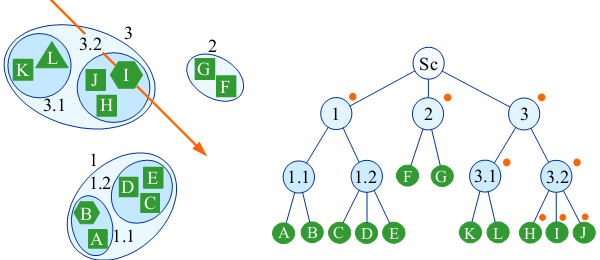
\includegraphics[width=0.6\textwidth]{assets/6_organizovani_do_struktur}
\end{figure}
\item Další metodou je \textbf{Dělení prostoru scény na podprostory}. Obykle se dělí rovinami souřadné soustavy $xy, xz, yz \,\to\,$ vznikají tak velké kvádry (stejně velké / různě velké). Princip metody:
\begin{itemize}
	\item u neurychlené metody byly všechny objekty organizovány v 1 velkém seznamu,
	\item nyní je zřízeno tolik seznamů, kolik je objemových elementů vzniklých dělením prostoru, každý element bude mít svůj seznam objektů, které do něj aspoň z části zasahují (pokud objekt zasahuje do více elementů, bude v seznamu každého z nich) -- hledání průsečíků začíná v tom elementu, kde je počátek paprsku, při opouštění elementu lze zjistit, do kterého elementu vstupuje, paprsek kontroluje pouze průsečíky s objekty, které jsou v seznamu daného elementu.
\end{itemize}
\begin{figure}[H]
\centering
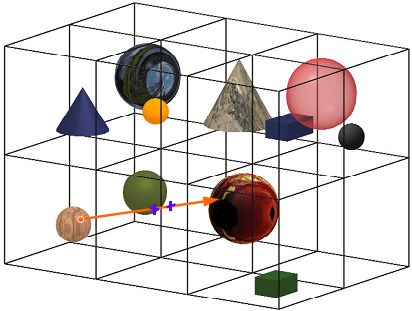
\includegraphics[width=0.4\textwidth]{assets/6_deleni_podprostor}
\end{figure}
\item Dalším metodou je \textbf{Adaptivní hloubka rekurze}. Odhaduje se, zda je paprsek pro stanovení intenzity ve zkoumaném obrazovém bodě dostatečně užitečný. Pokud ne, tak se nevyšle (např. u odrazů či průchodů tělesy).
% \item Protože je ray tracing výpočetně náročný, je vhodné jej urychlit.
% \item Nejjednodušší způsob je použití obalových struktur – bounding boxů.
% \item Ty mají nejčastěji tvar koule nebo osově zarovnaného kvádru (AABB).
% \item S jejich pomocí můžeme zjistit, zda se paprsek pohybuje v okolí objektu (tj. protíná strukturu).
% \item Pouze v případě, že ano, zjišťujeme jeho průsečíky s objektem.
% \item Vhodná obalová struktura má následující vlastnosti:
% 	\begin{itemize}
%		\item Objekt v ní vždy leží celý, ale struktura se jej snaží co nejvíce obepnout.
%		\item Co nejjednodušší výpočet pro ověření průsečíků s paprskem.
%		\item Dostatečně jednoduchá konstrukce.
%	\end{itemize}
\end{enumerate}
\subsection{Vyzařovací metoda - radiozita}
Na rozdíl od předchozí metody rekurzivního sledování paprsku (dobře zobrazuje lesklé, dobře osvícený předměty) je tato metoda spíše protikladná. Zaměřuje se na \textbf{difúzní odrazy světla} -- vhodná pro matné povrchy a rozptýlené světlo (např. interiéry). Princip:
\begin{itemize}
\item Vypočítá se, jak jsou osvětlena jednotlivá místa scény.
\item Podle toho se povrchy těles pokryjí sítí (v místech kde je komplikovaný průběh osvětlení je síť hustá -- zlom světla a stínu).
\item Pro každou plošku jsou spočítany hodnoty RGB -- vyzařování je konstantní na celém povrchu plošky.
\begin{itemize}
\item \textbf{PROBLÉM:} kdyby se takto plošky zobrazovaly, mohly by se sousedící plošky výrazně lišit intenzitou a nebylo by to pěkné.
\item 	\textbf{ŘEŠENÍ:} po výpočtu intenzit plošek se intenzity přenesou do jednotlivých uzlů sítě (zprůměrování intezit okolních plošek, které obklopují uzel) a následně se intenzity interpolují. (proto i to hustší dělení, kde je přechod světlo--stín ...).
\end{itemize}
\item Nejjednodušším, ale ne zrovna nejsprávnějším zobrazením scény a interpolací je pomocí \textbf{Gouradova stínování}. 
\begin{itemize}
	\item 	\textbf{PROBLÉM:} osvětlení bylo spočítáno v prostoru scény a tam by se měla provádět i interpolace, ale Gouraudovo stínování interpoluje v prostoru obrazu. Problém je, že při středové projekci se nezachovává dělící poměr a proto budou výsledky v prostoru obrazu rozdílné od výsledků z prostoru scény. Nicméně Gouraudovo stínování se používá, protože je rychlé.
\end{itemize}
\item Vytváření sítě probíhá v několika iteracích: nejdřív se hustota odhadne, pak se spočítá osvětlení a dle výsledků se síť dohustí tam, kde je třeba. Základní myšlenou je, že na všech ploškách ustanov \textbf{energetická rovnováha}: \textbf{ výkon vyzařovaný + výkon absorvovaný = výkon na plošku dopadající od jiných ploch + výkon, který ploška sama vyzařuje} 
\end{itemize}
\begin{equation*}
	B_i = E_i + p_i \sum\limits_{i=i}^n B_j F_{j \,\to\, i} \frac{A_j}{A_i}.
\end{equation*}
kde: 
\begin{itemize}
\item $B_j$ -- výkon vyzářený ploškou $j$,
\item $p_i$ -- míra odrazu (optické vlastnosti materiálu),
\item $E_i$ -- hodnota výkonu vlastního vyzařování plošky,
\item $A_i$,$A_j$ -- velikost plošek (plošný obsah),
\item $F_{j \,\to\, i}$ -- konfigurační koeficient říká, jaká část výkonu vyzářeného ploškou $j$ dopadne na plošku $i$ (jedná se o $\int \langle0,1\rangle$, záleží na pořadí indexů).
\end{itemize}
\begin{figure}[H]
\centering
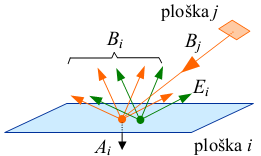
\includegraphics[width=0.4\textwidth]{assets/6_vyzarovaci_metoda}
\end{figure}

\subsection{BRDF (Bidirectional Reflectance Distribution Function)}
\begin{itemize}
	\item Charakterizuje \textbf{odrazové schopnosti povrchu materiálu} v určitém bodě $\mathbf{x}$.
	\item Jedná se o \textbf{poměr odraženého zářezí} ke vstupnímu diferenciálnímu zařízení, promítnutému na kolmou plochu.
	\item BRDF v daném bodě zůstává stejná i když změníme směr paprsku.
	\item \textbf{Pozitivita BRDF}: funkce není nikdy záporná.
	\item \textbf{Zákon zachování energie}: plocha nemůže odrazit víc než je celková přijatá energie
	\item \textbf{Odrazivost} $p(x) = \frac{d\Phi_r(x)}{d\Phi_i(x)}; \, d\Phi_r(x)$ je \textbf{odražený} světelný tok, $d\Phi_i(x)$ je \textbf{dopadající} světelný tok.
	\item Obor hodnot odrazivosti je na intervalu $<0,1>, \, 1=$ \textbf{plný odraz}.
	\item \textbf{PRINCIP:} Vysílá se mnoho paprsků v každém bodě s různými offsety, některé padnou do zdroje světla, některé ne. Výsledná hodnota pixelu je poté průměrem všech hodnot paprsků (čím více paprsků vyšleme, čím lepší je výsledek (méně zrní)).
\end{itemize}
\begin{figure}[H]
\centering
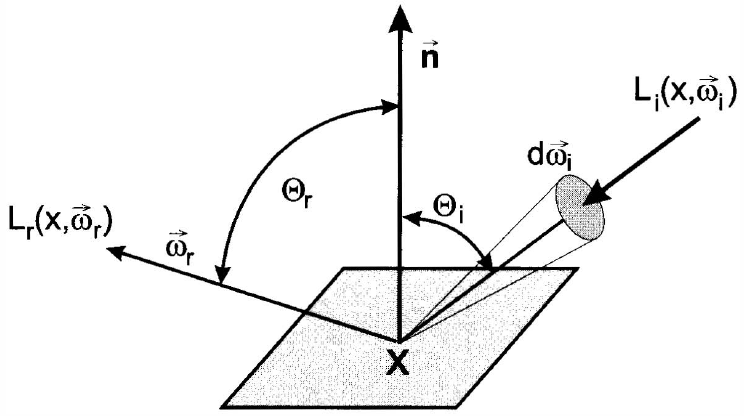
\includegraphics[width=0.4\textwidth]{assets/6_brdf}
\end{figure}
\subsection{BTDF (Bidirectional Transmittance Distribution Function)}
Dvousměrná distribuční fuknce lomu. Popisuje \textbf{průchod světla povrchem}.

\subsection{BSDF (Bidirectional Scattering Distribution Function)}
\begin{itemize}
	\item Obousměrná distribuční funkce \textbf{rozptylu}.
	\item Je to souhrn dvou distribučních fukncí, a to funkce odrazu (BRDF) a lomu (BTDF).
	\item \textbf{BSDF + BTDF + BRDF}
\end{itemize}
\begin{figure}[H]
\centering
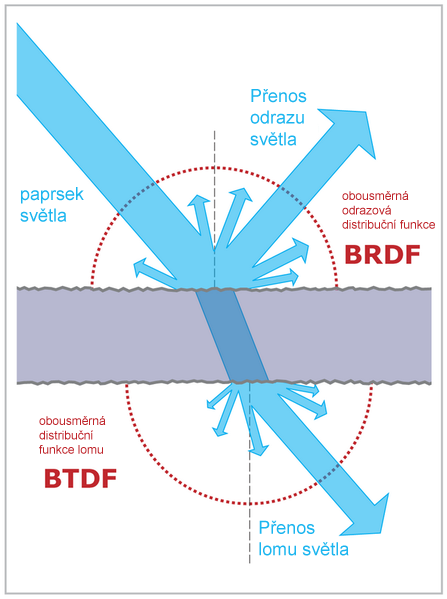
\includegraphics[width=0.4\textwidth]{assets/6_bsdf}
\end{figure}


\subsection{Renderovací rovnice}
Rekurzivní diferenciální rovnice
\begin{equation*}
	L(x, \omega_0) = L_e(x,\omega_0) + \int_{\Omega} L(r(x,\omega_i) - \omega_i) \cdot BRDF(\omega_i,x,\omega_0) \cos{\theta_id\omega_i}
\end{equation*}
Zjednodušeně: \textbf{osvětlení povrchu = samovolně vyzařované světlo + součet příchozího osvěrlení ze všech směrů krát BRDF}.